\documentclass[12pt, letterpaper]{report}
\usepackage[utf8]{inputenc}
\usepackage[T1]{fontenc}
\usepackage[a4paper,left=2cm,right=2cm,top=2cm,bottom=2cm]{geometry}
\usepackage{booktabs}
\usepackage[french]{babel}
\usepackage{libertine}
\usepackage[pdftex]{graphicx}
\usepackage{csquotes}
\usepackage{url}
\usepackage{hyperref}
\hypersetup{colorlinks=true,linkcolor=black}


\setlength{\parskip}{1em}
\setlength{\parindent}{0em}
\newcommand{\hsp}{\hspace{20pt}}
\newcommand{\HRule}{\rule{\linewidth}{0.5mm}}

\begin{document}
\begin{titlepage}
  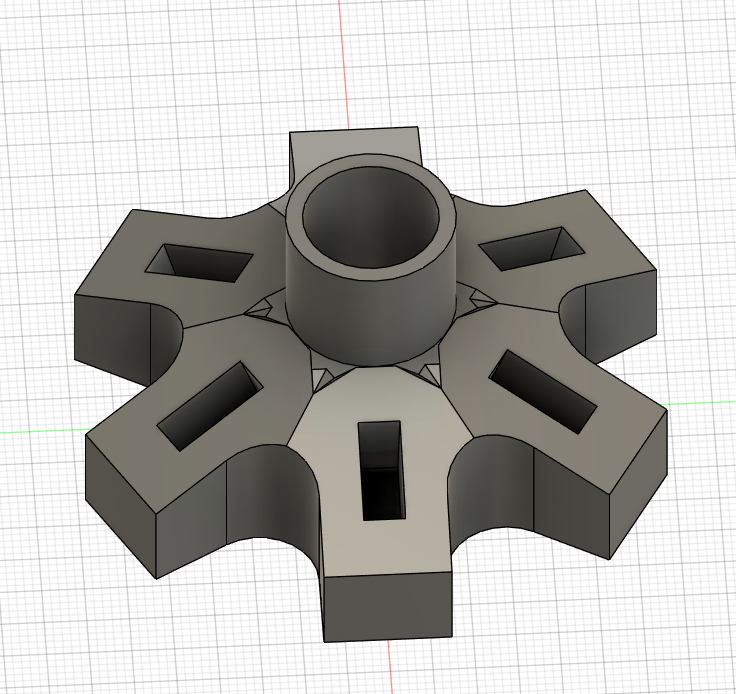
\includegraphics[scale=0.7]{IMG1.JPG}
  \begin{sffamily}
    \begin{center}


      \textsc{\LARGE Henallux - Institut d'enseignement supérieur de Namur}\[2cm]

        \textsc{\Large Laboratoire de sciences appliquées à l'informatique}\[1.5cm]

          \HRule \[0.4cm]
            \huge \bfseries {Laboratoire \#01 - Analyse de signaux \[0.4cm]}
              \HRule \[2cm]

                \begin{minipage}{0.4\textwidth}
                  \begin{flushleft} \large
                    Schoonjans \textsc{Ludovic}\
                    Vanderbeken  \textsc{Mathias}\
                    Dubois  \textsc{Aaron}\
                    Combette  \textsc{Nathan}\
                  \end{flushleft}
                \end{minipage}
                \begin{minipage}{0.4\textwidth}
                  \begin{flushright} \large
                    \emph{Professeur :} \textsc{Guillerme Duvillié}\
                    \emph{Groupe :} \textsc{Les coléoptères \du frigos}\
                  \end{flushright}
                \end{minipage}

                \vfill

                \large 18 Avril 2023
    \end{center}
  \end{sffamily}
\end{titlepage}

\renewcommand*\contentsname{Table des matières}
\tableofcontents

\chapter{Introduction}
L'objectif principal de ce rapport est d'étudier les séries de Fourier et leur application dans l'analyse de signaux périodiques complexes. Plus précisément, ce rapport vise à:

    Comprendre les bases théoriques des séries de Fourier.
    Appliquer les séries de Fourier pour décomposer et reconstruire des signaux complexes.
    Analyser les signaux obtenus et discuter des limitations éventuelles.
\chapter{Matériel utilisé}
 Pour mener à bien ce travail, le logiciel Audacity a été utilisé pour générer et manipuler des signaux sinusoïdaux à différentes fréquences et amplitudes. Le spectre de fréquences a été analysé pour vérifier la décomposition et la reconstruction des signaux.

\chapter{Notions théoriques}
Les séries de Fourier sont basées sur l'idée que tout signal périodique peut être décomposé en une somme de signaux sinusoïdaux de fréquences et d'amplitudes différentes. Cette décomposition permet d'étudier les signaux complexes et de déterminer les fréquences les plus présentes dans le signal.


\chapter{Manipulation}
\section{Préparation}
\section{Signal carré}
L'application des séries de Fourier au signal carré a montré que le signal reconstruit se rapproche du signal carré original. L'analyse du spectre de fréquences a confirmé la présence des fréquences et amplitudes utilisées pour la reconstruction.
\section{Signal triangulaire}
Le signal triangulaire a également été reconstruit en utilisant les séries de Fourier. Bien que le signal obtenu ne soit pas parfait, il présente une tendance similaire au signal triangulaire original. L'analyse du spectre de fréquences a confirmé la présence des fréquences et amplitudes utilisées pour la reconstruction.
\section{Signal en "vague"}
Un signal en "vague" a été tenté en utilisant dix signaux sinusoïdaux de fréquences et d'amplitudes différentes. Le signal reconstruit présente une corrélation avec le signal théorique, bien qu'il ne soit pas parfaitement identique.
\chapter{constatation}
Les résultats obtenus montrent que les séries de Fourier sont un outil efficace pour décomposer et reconstruire des signaux périodiques complexes. Dans chaque cas étudié (signal carré, signal triangulaire et signal en "vague"), la reconstruction des signaux à l'aide des séries de Fourier a produit des résultats similaires aux signaux originaux. L'analyse du spectre de fréquences a également confirmé la présence des fréquences et amplitudes utilisées pour la reconstruction.

Cependant, il convient de noter que les signaux reconstruits ne sont pas toujours identiques aux signaux originaux. Cela peut être dû à plusieurs facteurs, tels que les limitations du logiciel Audacity, les imprécisions dans le traitement des données et le fait que la décomposition en séries de Fourier nécessite un nombre infini de termes pour reproduire parfaitement un signal périodique. Néanmoins, les résultats obtenus sont suffisamment proches pour démontrer l'utilité des séries de Fourier dans l'analyse des signaux complexes.

Il est également important de mentionner que les séries de Fourier ne sont pas limitées à l'analyse des signaux audibles. Elles peuvent être appliquées à d'autres domaines, tels que l'imagerie médicale, la télécommunication et d'autres domaines scientifiques où l'analyse des signaux périodiques est nécessaire.
\chapter{Conclusion}
L'étude des séries de Fourier et leur application dans l'analyse de signaux périodiques complexes ont montré que cette méthode est efficace pour décomposer et reconstruire des signaux complexes en une somme de signaux sinusoïdaux plus simples. Les résultats obtenus sont encourageants et confirment l'utilité des séries de Fourier dans diverses applications, pas seulement en télécommunication, mais également en imagerie médicale et dans d'autres domaines scientifiques. Bien que les signaux reconstruits ne soient pas toujours identiques aux signaux originaux, ils sont suffisamment proches pour valider cette méthode d'analyse.
\chapter{Bibliographie}

$[Fig.2.1]$ {}

$[1]$ \textsc{Wikipédia}, \emph{Loi d'Ohm}, \newline
{},\quad consulté le 03/04/2023 à 14h43.
\smallskip

$[2]$ \textsc{Wikipédia}, \emph{Décibel}, \newline
{},\quad consulté le 03/04/2023 à 14h02.
\smallskip

$[3]$ \textsc{Wikipédia}, \emph{Énergie électrique},\newline
{},\quad consulté le 03/04/2023 à 14h47.

\end{document}
